%% AMS-LaTeX Created with the Wolfram Language for Students - Personal Use Only : www.wolfram.com

\documentclass{article}
\usepackage{amsmath, amssymb, graphics, setspace}

\newcommand{\mathsym}[1]{{}}
\newcommand{\unicode}[1]{{}}

\newcounter{mathematicapage}
\begin{document}

\\
1

\begin{doublespace}
\noindent\(\pmb{\text{SQRmatrixSize}=10;}\\
\pmb{\text{matrixAentries} =\text{Range}[1,\text{SQRmatrixSize}*\text{SQRmatrixSize}];}\\
\pmb{\text{matrixAentries}=\text{ArrayReshape}[\text{matrixAentries},\{\text{SQRmatrixSize},\text{SQRmatrixSize}\}];}\\
\pmb{\text{matrixA}=\text{Table}[\text{matrixAentries}[[i,j]],\{i,1,\text{SQRmatrixSize}\},\{j,1,\text{SQRmatrixSize}\}];}\\
\pmb{\text{MatrixForm}[\text{matrixA}]}\)
\end{doublespace}

\begin{doublespace}
\noindent\(\left(
\begin{array}{cccccccccc}
 1 & 2 & 3 & 4 & 5 & 6 & 7 & 8 & 9 & 10 \\
 11 & 12 & 13 & 14 & 15 & 16 & 17 & 18 & 19 & 20 \\
 21 & 22 & 23 & 24 & 25 & 26 & 27 & 28 & 29 & 30 \\
 31 & 32 & 33 & 34 & 35 & 36 & 37 & 38 & 39 & 40 \\
 41 & 42 & 43 & 44 & 45 & 46 & 47 & 48 & 49 & 50 \\
 51 & 52 & 53 & 54 & 55 & 56 & 57 & 58 & 59 & 60 \\
 61 & 62 & 63 & 64 & 65 & 66 & 67 & 68 & 69 & 70 \\
 71 & 72 & 73 & 74 & 75 & 76 & 77 & 78 & 79 & 80 \\
 81 & 82 & 83 & 84 & 85 & 86 & 87 & 88 & 89 & 90 \\
 91 & 92 & 93 & 94 & 95 & 96 & 97 & 98 & 99 & 100 \\
\end{array}
\right)\)
\end{doublespace}

\\
2\\
matrixA is singular, therefore Inverse[matrixA] does not exist.

\\
3

\begin{doublespace}
\noindent\(\pmb{\text{SQRmatrixSize}=30;}\\
\pmb{\text{matrixB}=\pi *\text{IdentityMatrix}[\text{SQRmatrixSize}];}\\
\pmb{\text{MatrixForm}[\text{matrixB}]}\)
\end{doublespace}

\begin{doublespace}
\noindent\(\left(
\begin{array}{cccccccccccccccccccccccccccccc}
 \pi  & 0 & 0 & 0 & 0 & 0 & 0 & 0 & 0 & 0 & 0 & 0 & 0 & 0 & 0 & 0 & 0 & 0 & 0 & 0 & 0 & 0 & 0 & 0 & 0 & 0 & 0 & 0 & 0 & 0 \\
 0 & \pi  & 0 & 0 & 0 & 0 & 0 & 0 & 0 & 0 & 0 & 0 & 0 & 0 & 0 & 0 & 0 & 0 & 0 & 0 & 0 & 0 & 0 & 0 & 0 & 0 & 0 & 0 & 0 & 0 \\
 0 & 0 & \pi  & 0 & 0 & 0 & 0 & 0 & 0 & 0 & 0 & 0 & 0 & 0 & 0 & 0 & 0 & 0 & 0 & 0 & 0 & 0 & 0 & 0 & 0 & 0 & 0 & 0 & 0 & 0 \\
 0 & 0 & 0 & \pi  & 0 & 0 & 0 & 0 & 0 & 0 & 0 & 0 & 0 & 0 & 0 & 0 & 0 & 0 & 0 & 0 & 0 & 0 & 0 & 0 & 0 & 0 & 0 & 0 & 0 & 0 \\
 0 & 0 & 0 & 0 & \pi  & 0 & 0 & 0 & 0 & 0 & 0 & 0 & 0 & 0 & 0 & 0 & 0 & 0 & 0 & 0 & 0 & 0 & 0 & 0 & 0 & 0 & 0 & 0 & 0 & 0 \\
 0 & 0 & 0 & 0 & 0 & \pi  & 0 & 0 & 0 & 0 & 0 & 0 & 0 & 0 & 0 & 0 & 0 & 0 & 0 & 0 & 0 & 0 & 0 & 0 & 0 & 0 & 0 & 0 & 0 & 0 \\
 0 & 0 & 0 & 0 & 0 & 0 & \pi  & 0 & 0 & 0 & 0 & 0 & 0 & 0 & 0 & 0 & 0 & 0 & 0 & 0 & 0 & 0 & 0 & 0 & 0 & 0 & 0 & 0 & 0 & 0 \\
 0 & 0 & 0 & 0 & 0 & 0 & 0 & \pi  & 0 & 0 & 0 & 0 & 0 & 0 & 0 & 0 & 0 & 0 & 0 & 0 & 0 & 0 & 0 & 0 & 0 & 0 & 0 & 0 & 0 & 0 \\
 0 & 0 & 0 & 0 & 0 & 0 & 0 & 0 & \pi  & 0 & 0 & 0 & 0 & 0 & 0 & 0 & 0 & 0 & 0 & 0 & 0 & 0 & 0 & 0 & 0 & 0 & 0 & 0 & 0 & 0 \\
 0 & 0 & 0 & 0 & 0 & 0 & 0 & 0 & 0 & \pi  & 0 & 0 & 0 & 0 & 0 & 0 & 0 & 0 & 0 & 0 & 0 & 0 & 0 & 0 & 0 & 0 & 0 & 0 & 0 & 0 \\
 0 & 0 & 0 & 0 & 0 & 0 & 0 & 0 & 0 & 0 & \pi  & 0 & 0 & 0 & 0 & 0 & 0 & 0 & 0 & 0 & 0 & 0 & 0 & 0 & 0 & 0 & 0 & 0 & 0 & 0 \\
 0 & 0 & 0 & 0 & 0 & 0 & 0 & 0 & 0 & 0 & 0 & \pi  & 0 & 0 & 0 & 0 & 0 & 0 & 0 & 0 & 0 & 0 & 0 & 0 & 0 & 0 & 0 & 0 & 0 & 0 \\
 0 & 0 & 0 & 0 & 0 & 0 & 0 & 0 & 0 & 0 & 0 & 0 & \pi  & 0 & 0 & 0 & 0 & 0 & 0 & 0 & 0 & 0 & 0 & 0 & 0 & 0 & 0 & 0 & 0 & 0 \\
 0 & 0 & 0 & 0 & 0 & 0 & 0 & 0 & 0 & 0 & 0 & 0 & 0 & \pi  & 0 & 0 & 0 & 0 & 0 & 0 & 0 & 0 & 0 & 0 & 0 & 0 & 0 & 0 & 0 & 0 \\
 0 & 0 & 0 & 0 & 0 & 0 & 0 & 0 & 0 & 0 & 0 & 0 & 0 & 0 & \pi  & 0 & 0 & 0 & 0 & 0 & 0 & 0 & 0 & 0 & 0 & 0 & 0 & 0 & 0 & 0 \\
 0 & 0 & 0 & 0 & 0 & 0 & 0 & 0 & 0 & 0 & 0 & 0 & 0 & 0 & 0 & \pi  & 0 & 0 & 0 & 0 & 0 & 0 & 0 & 0 & 0 & 0 & 0 & 0 & 0 & 0 \\
 0 & 0 & 0 & 0 & 0 & 0 & 0 & 0 & 0 & 0 & 0 & 0 & 0 & 0 & 0 & 0 & \pi  & 0 & 0 & 0 & 0 & 0 & 0 & 0 & 0 & 0 & 0 & 0 & 0 & 0 \\
 0 & 0 & 0 & 0 & 0 & 0 & 0 & 0 & 0 & 0 & 0 & 0 & 0 & 0 & 0 & 0 & 0 & \pi  & 0 & 0 & 0 & 0 & 0 & 0 & 0 & 0 & 0 & 0 & 0 & 0 \\
 0 & 0 & 0 & 0 & 0 & 0 & 0 & 0 & 0 & 0 & 0 & 0 & 0 & 0 & 0 & 0 & 0 & 0 & \pi  & 0 & 0 & 0 & 0 & 0 & 0 & 0 & 0 & 0 & 0 & 0 \\
 0 & 0 & 0 & 0 & 0 & 0 & 0 & 0 & 0 & 0 & 0 & 0 & 0 & 0 & 0 & 0 & 0 & 0 & 0 & \pi  & 0 & 0 & 0 & 0 & 0 & 0 & 0 & 0 & 0 & 0 \\
 0 & 0 & 0 & 0 & 0 & 0 & 0 & 0 & 0 & 0 & 0 & 0 & 0 & 0 & 0 & 0 & 0 & 0 & 0 & 0 & \pi  & 0 & 0 & 0 & 0 & 0 & 0 & 0 & 0 & 0 \\
 0 & 0 & 0 & 0 & 0 & 0 & 0 & 0 & 0 & 0 & 0 & 0 & 0 & 0 & 0 & 0 & 0 & 0 & 0 & 0 & 0 & \pi  & 0 & 0 & 0 & 0 & 0 & 0 & 0 & 0 \\
 0 & 0 & 0 & 0 & 0 & 0 & 0 & 0 & 0 & 0 & 0 & 0 & 0 & 0 & 0 & 0 & 0 & 0 & 0 & 0 & 0 & 0 & \pi  & 0 & 0 & 0 & 0 & 0 & 0 & 0 \\
 0 & 0 & 0 & 0 & 0 & 0 & 0 & 0 & 0 & 0 & 0 & 0 & 0 & 0 & 0 & 0 & 0 & 0 & 0 & 0 & 0 & 0 & 0 & \pi  & 0 & 0 & 0 & 0 & 0 & 0 \\
 0 & 0 & 0 & 0 & 0 & 0 & 0 & 0 & 0 & 0 & 0 & 0 & 0 & 0 & 0 & 0 & 0 & 0 & 0 & 0 & 0 & 0 & 0 & 0 & \pi  & 0 & 0 & 0 & 0 & 0 \\
 0 & 0 & 0 & 0 & 0 & 0 & 0 & 0 & 0 & 0 & 0 & 0 & 0 & 0 & 0 & 0 & 0 & 0 & 0 & 0 & 0 & 0 & 0 & 0 & 0 & \pi  & 0 & 0 & 0 & 0 \\
 0 & 0 & 0 & 0 & 0 & 0 & 0 & 0 & 0 & 0 & 0 & 0 & 0 & 0 & 0 & 0 & 0 & 0 & 0 & 0 & 0 & 0 & 0 & 0 & 0 & 0 & \pi  & 0 & 0 & 0 \\
 0 & 0 & 0 & 0 & 0 & 0 & 0 & 0 & 0 & 0 & 0 & 0 & 0 & 0 & 0 & 0 & 0 & 0 & 0 & 0 & 0 & 0 & 0 & 0 & 0 & 0 & 0 & \pi  & 0 & 0 \\
 0 & 0 & 0 & 0 & 0 & 0 & 0 & 0 & 0 & 0 & 0 & 0 & 0 & 0 & 0 & 0 & 0 & 0 & 0 & 0 & 0 & 0 & 0 & 0 & 0 & 0 & 0 & 0 & \pi  & 0 \\
 0 & 0 & 0 & 0 & 0 & 0 & 0 & 0 & 0 & 0 & 0 & 0 & 0 & 0 & 0 & 0 & 0 & 0 & 0 & 0 & 0 & 0 & 0 & 0 & 0 & 0 & 0 & 0 & 0 & \pi  \\
\end{array}
\right)\)
\end{doublespace}

\\
3.a $\&$ 3.b\\
Yes, {``}A triangular matrix (upper, lower or diagonal) is invertible if and only if no element on its main diagonal is 0.{''}\\
\\
{``}by hand{''} ...\\
Since, Inverse[A] equals diag(\(\frac{1}{a_1},\frac{1}{a_2},\ldots ,\frac{1}{a_n}\)), Inverse[matrixB] is equal to \(\(\frac{1}{\pi }\)\)IdentityMatrix[30]\\
\\
Verification with Mathematica is shown below ...

\begin{doublespace}
\noindent\(\pmb{\text{Inverse}[\text{matrixB}];}\\
\pmb{\text{MatrixForm}[\%]}\)
\end{doublespace}

\begin{doublespace}
\noindent\(\left(
\begin{array}{cccccccccccccccccccccccccccccc}
 \frac{1}{\pi } & 0 & 0 & 0 & 0 & 0 & 0 & 0 & 0 & 0 & 0 & 0 & 0 & 0 & 0 & 0 & 0 & 0 & 0 & 0 & 0 & 0 & 0 & 0 & 0 & 0 & 0 & 0 & 0 & 0 \\
 0 & \frac{1}{\pi } & 0 & 0 & 0 & 0 & 0 & 0 & 0 & 0 & 0 & 0 & 0 & 0 & 0 & 0 & 0 & 0 & 0 & 0 & 0 & 0 & 0 & 0 & 0 & 0 & 0 & 0 & 0 & 0 \\
 0 & 0 & \frac{1}{\pi } & 0 & 0 & 0 & 0 & 0 & 0 & 0 & 0 & 0 & 0 & 0 & 0 & 0 & 0 & 0 & 0 & 0 & 0 & 0 & 0 & 0 & 0 & 0 & 0 & 0 & 0 & 0 \\
 0 & 0 & 0 & \frac{1}{\pi } & 0 & 0 & 0 & 0 & 0 & 0 & 0 & 0 & 0 & 0 & 0 & 0 & 0 & 0 & 0 & 0 & 0 & 0 & 0 & 0 & 0 & 0 & 0 & 0 & 0 & 0 \\
 0 & 0 & 0 & 0 & \frac{1}{\pi } & 0 & 0 & 0 & 0 & 0 & 0 & 0 & 0 & 0 & 0 & 0 & 0 & 0 & 0 & 0 & 0 & 0 & 0 & 0 & 0 & 0 & 0 & 0 & 0 & 0 \\
 0 & 0 & 0 & 0 & 0 & \frac{1}{\pi } & 0 & 0 & 0 & 0 & 0 & 0 & 0 & 0 & 0 & 0 & 0 & 0 & 0 & 0 & 0 & 0 & 0 & 0 & 0 & 0 & 0 & 0 & 0 & 0 \\
 0 & 0 & 0 & 0 & 0 & 0 & \frac{1}{\pi } & 0 & 0 & 0 & 0 & 0 & 0 & 0 & 0 & 0 & 0 & 0 & 0 & 0 & 0 & 0 & 0 & 0 & 0 & 0 & 0 & 0 & 0 & 0 \\
 0 & 0 & 0 & 0 & 0 & 0 & 0 & \frac{1}{\pi } & 0 & 0 & 0 & 0 & 0 & 0 & 0 & 0 & 0 & 0 & 0 & 0 & 0 & 0 & 0 & 0 & 0 & 0 & 0 & 0 & 0 & 0 \\
 0 & 0 & 0 & 0 & 0 & 0 & 0 & 0 & \frac{1}{\pi } & 0 & 0 & 0 & 0 & 0 & 0 & 0 & 0 & 0 & 0 & 0 & 0 & 0 & 0 & 0 & 0 & 0 & 0 & 0 & 0 & 0 \\
 0 & 0 & 0 & 0 & 0 & 0 & 0 & 0 & 0 & \frac{1}{\pi } & 0 & 0 & 0 & 0 & 0 & 0 & 0 & 0 & 0 & 0 & 0 & 0 & 0 & 0 & 0 & 0 & 0 & 0 & 0 & 0 \\
 0 & 0 & 0 & 0 & 0 & 0 & 0 & 0 & 0 & 0 & \frac{1}{\pi } & 0 & 0 & 0 & 0 & 0 & 0 & 0 & 0 & 0 & 0 & 0 & 0 & 0 & 0 & 0 & 0 & 0 & 0 & 0 \\
 0 & 0 & 0 & 0 & 0 & 0 & 0 & 0 & 0 & 0 & 0 & \frac{1}{\pi } & 0 & 0 & 0 & 0 & 0 & 0 & 0 & 0 & 0 & 0 & 0 & 0 & 0 & 0 & 0 & 0 & 0 & 0 \\
 0 & 0 & 0 & 0 & 0 & 0 & 0 & 0 & 0 & 0 & 0 & 0 & \frac{1}{\pi } & 0 & 0 & 0 & 0 & 0 & 0 & 0 & 0 & 0 & 0 & 0 & 0 & 0 & 0 & 0 & 0 & 0 \\
 0 & 0 & 0 & 0 & 0 & 0 & 0 & 0 & 0 & 0 & 0 & 0 & 0 & \frac{1}{\pi } & 0 & 0 & 0 & 0 & 0 & 0 & 0 & 0 & 0 & 0 & 0 & 0 & 0 & 0 & 0 & 0 \\
 0 & 0 & 0 & 0 & 0 & 0 & 0 & 0 & 0 & 0 & 0 & 0 & 0 & 0 & \frac{1}{\pi } & 0 & 0 & 0 & 0 & 0 & 0 & 0 & 0 & 0 & 0 & 0 & 0 & 0 & 0 & 0 \\
 0 & 0 & 0 & 0 & 0 & 0 & 0 & 0 & 0 & 0 & 0 & 0 & 0 & 0 & 0 & \frac{1}{\pi } & 0 & 0 & 0 & 0 & 0 & 0 & 0 & 0 & 0 & 0 & 0 & 0 & 0 & 0 \\
 0 & 0 & 0 & 0 & 0 & 0 & 0 & 0 & 0 & 0 & 0 & 0 & 0 & 0 & 0 & 0 & \frac{1}{\pi } & 0 & 0 & 0 & 0 & 0 & 0 & 0 & 0 & 0 & 0 & 0 & 0 & 0 \\
 0 & 0 & 0 & 0 & 0 & 0 & 0 & 0 & 0 & 0 & 0 & 0 & 0 & 0 & 0 & 0 & 0 & \frac{1}{\pi } & 0 & 0 & 0 & 0 & 0 & 0 & 0 & 0 & 0 & 0 & 0 & 0 \\
 0 & 0 & 0 & 0 & 0 & 0 & 0 & 0 & 0 & 0 & 0 & 0 & 0 & 0 & 0 & 0 & 0 & 0 & \frac{1}{\pi } & 0 & 0 & 0 & 0 & 0 & 0 & 0 & 0 & 0 & 0 & 0 \\
 0 & 0 & 0 & 0 & 0 & 0 & 0 & 0 & 0 & 0 & 0 & 0 & 0 & 0 & 0 & 0 & 0 & 0 & 0 & \frac{1}{\pi } & 0 & 0 & 0 & 0 & 0 & 0 & 0 & 0 & 0 & 0 \\
 0 & 0 & 0 & 0 & 0 & 0 & 0 & 0 & 0 & 0 & 0 & 0 & 0 & 0 & 0 & 0 & 0 & 0 & 0 & 0 & \frac{1}{\pi } & 0 & 0 & 0 & 0 & 0 & 0 & 0 & 0 & 0 \\
 0 & 0 & 0 & 0 & 0 & 0 & 0 & 0 & 0 & 0 & 0 & 0 & 0 & 0 & 0 & 0 & 0 & 0 & 0 & 0 & 0 & \frac{1}{\pi } & 0 & 0 & 0 & 0 & 0 & 0 & 0 & 0 \\
 0 & 0 & 0 & 0 & 0 & 0 & 0 & 0 & 0 & 0 & 0 & 0 & 0 & 0 & 0 & 0 & 0 & 0 & 0 & 0 & 0 & 0 & \frac{1}{\pi } & 0 & 0 & 0 & 0 & 0 & 0 & 0 \\
 0 & 0 & 0 & 0 & 0 & 0 & 0 & 0 & 0 & 0 & 0 & 0 & 0 & 0 & 0 & 0 & 0 & 0 & 0 & 0 & 0 & 0 & 0 & \frac{1}{\pi } & 0 & 0 & 0 & 0 & 0 & 0 \\
 0 & 0 & 0 & 0 & 0 & 0 & 0 & 0 & 0 & 0 & 0 & 0 & 0 & 0 & 0 & 0 & 0 & 0 & 0 & 0 & 0 & 0 & 0 & 0 & \frac{1}{\pi } & 0 & 0 & 0 & 0 & 0 \\
 0 & 0 & 0 & 0 & 0 & 0 & 0 & 0 & 0 & 0 & 0 & 0 & 0 & 0 & 0 & 0 & 0 & 0 & 0 & 0 & 0 & 0 & 0 & 0 & 0 & \frac{1}{\pi } & 0 & 0 & 0 & 0 \\
 0 & 0 & 0 & 0 & 0 & 0 & 0 & 0 & 0 & 0 & 0 & 0 & 0 & 0 & 0 & 0 & 0 & 0 & 0 & 0 & 0 & 0 & 0 & 0 & 0 & 0 & \frac{1}{\pi } & 0 & 0 & 0 \\
 0 & 0 & 0 & 0 & 0 & 0 & 0 & 0 & 0 & 0 & 0 & 0 & 0 & 0 & 0 & 0 & 0 & 0 & 0 & 0 & 0 & 0 & 0 & 0 & 0 & 0 & 0 & \frac{1}{\pi } & 0 & 0 \\
 0 & 0 & 0 & 0 & 0 & 0 & 0 & 0 & 0 & 0 & 0 & 0 & 0 & 0 & 0 & 0 & 0 & 0 & 0 & 0 & 0 & 0 & 0 & 0 & 0 & 0 & 0 & 0 & \frac{1}{\pi } & 0 \\
 0 & 0 & 0 & 0 & 0 & 0 & 0 & 0 & 0 & 0 & 0 & 0 & 0 & 0 & 0 & 0 & 0 & 0 & 0 & 0 & 0 & 0 & 0 & 0 & 0 & 0 & 0 & 0 & 0 & \frac{1}{\pi } \\
\end{array}
\right)\)
\end{doublespace}

\\
3.c

\begin{doublespace}
\noindent\(\pmb{\text{MatrixRank}[\text{matrixB}]}\)
\end{doublespace}

\begin{doublespace}
\noindent\(30\)
\end{doublespace}

\\
4

\begin{doublespace}
\noindent\(\pmb{\text{SQRmatrixSize}=16;}\\
\pmb{\text{matrixC}=\text{Table}[0,\{i,1,\text{SQRmatrixSize}\},\{j,1,\text{SQRmatrixSize}\}];}\\
\pmb{\text{rows}=\text{Dimensions}[\text{matrixC}][[1]];}\\
\pmb{\text{cols}=\text{Dimensions}[\text{matrixC}][[2]];}\\
\pmb{\text{For}[i=1,i\leq  \text{rows},i\text{++},}\\
\pmb{\text{For}[j=1,j\leq  \text{cols},j\text{++},}\\
\pmb{\text{If}[i==j,}\\
\pmb{\text{matrixC}[[i,j]]=(\pi +i)-1,}\\
\pmb{\text{matrixC}[[i,j]]=0];}\\
\pmb{];}\\
\pmb{];}\\
\pmb{\text{MatrixForm}[\text{matrixC}]}\)
\end{doublespace}

\begin{doublespace}
\noindent\(\left(
\begin{array}{cccccccccccccccc}
 \pi  & 0 & 0 & 0 & 0 & 0 & 0 & 0 & 0 & 0 & 0 & 0 & 0 & 0 & 0 & 0 \\
 0 & 1+\pi  & 0 & 0 & 0 & 0 & 0 & 0 & 0 & 0 & 0 & 0 & 0 & 0 & 0 & 0 \\
 0 & 0 & 2+\pi  & 0 & 0 & 0 & 0 & 0 & 0 & 0 & 0 & 0 & 0 & 0 & 0 & 0 \\
 0 & 0 & 0 & 3+\pi  & 0 & 0 & 0 & 0 & 0 & 0 & 0 & 0 & 0 & 0 & 0 & 0 \\
 0 & 0 & 0 & 0 & 4+\pi  & 0 & 0 & 0 & 0 & 0 & 0 & 0 & 0 & 0 & 0 & 0 \\
 0 & 0 & 0 & 0 & 0 & 5+\pi  & 0 & 0 & 0 & 0 & 0 & 0 & 0 & 0 & 0 & 0 \\
 0 & 0 & 0 & 0 & 0 & 0 & 6+\pi  & 0 & 0 & 0 & 0 & 0 & 0 & 0 & 0 & 0 \\
 0 & 0 & 0 & 0 & 0 & 0 & 0 & 7+\pi  & 0 & 0 & 0 & 0 & 0 & 0 & 0 & 0 \\
 0 & 0 & 0 & 0 & 0 & 0 & 0 & 0 & 8+\pi  & 0 & 0 & 0 & 0 & 0 & 0 & 0 \\
 0 & 0 & 0 & 0 & 0 & 0 & 0 & 0 & 0 & 9+\pi  & 0 & 0 & 0 & 0 & 0 & 0 \\
 0 & 0 & 0 & 0 & 0 & 0 & 0 & 0 & 0 & 0 & 10+\pi  & 0 & 0 & 0 & 0 & 0 \\
 0 & 0 & 0 & 0 & 0 & 0 & 0 & 0 & 0 & 0 & 0 & 11+\pi  & 0 & 0 & 0 & 0 \\
 0 & 0 & 0 & 0 & 0 & 0 & 0 & 0 & 0 & 0 & 0 & 0 & 12+\pi  & 0 & 0 & 0 \\
 0 & 0 & 0 & 0 & 0 & 0 & 0 & 0 & 0 & 0 & 0 & 0 & 0 & 13+\pi  & 0 & 0 \\
 0 & 0 & 0 & 0 & 0 & 0 & 0 & 0 & 0 & 0 & 0 & 0 & 0 & 0 & 14+\pi  & 0 \\
 0 & 0 & 0 & 0 & 0 & 0 & 0 & 0 & 0 & 0 & 0 & 0 & 0 & 0 & 0 & 15+\pi  \\
\end{array}
\right)\)
\end{doublespace}

\\
4.a $\&$ 4.b\\
Yes, {``}A triangular matrix (upper, lower or diagonal) is invertible if and only if no element on its main diagonal is 0.{''}\\
\\
{``}by hand{''} ...\\
Since, Inverse[A] equals diag(\(\frac{1}{a_1},\frac{1}{a_2},\ldots ,\frac{1}{a_n}\)), Inverse[matrixB] is equal to \(\(\frac{1}{(\pi +i)-1}\)\)IdentityMatrix[16]\\
\\
Verification with Mathematica is shown below ...

\begin{doublespace}
\noindent\(\pmb{\text{Inverse}[\text{matrixC}];}\\
\pmb{\text{MatrixForm}[\%]}\)
\end{doublespace}

\begin{doublespace}
\noindent\(\left(
\begin{array}{cccccccccccccccc}
 \frac{1}{\pi } & 0 & 0 & 0 & 0 & 0 & 0 & 0 & 0 & 0 & 0 & 0 & 0 & 0 & 0 & 0 \\
 0 & \frac{1}{1+\pi } & 0 & 0 & 0 & 0 & 0 & 0 & 0 & 0 & 0 & 0 & 0 & 0 & 0 & 0 \\
 0 & 0 & \frac{1}{2+\pi } & 0 & 0 & 0 & 0 & 0 & 0 & 0 & 0 & 0 & 0 & 0 & 0 & 0 \\
 0 & 0 & 0 & \frac{1}{3+\pi } & 0 & 0 & 0 & 0 & 0 & 0 & 0 & 0 & 0 & 0 & 0 & 0 \\
 0 & 0 & 0 & 0 & \frac{1}{4+\pi } & 0 & 0 & 0 & 0 & 0 & 0 & 0 & 0 & 0 & 0 & 0 \\
 0 & 0 & 0 & 0 & 0 & \frac{1}{5+\pi } & 0 & 0 & 0 & 0 & 0 & 0 & 0 & 0 & 0 & 0 \\
 0 & 0 & 0 & 0 & 0 & 0 & \frac{1}{6+\pi } & 0 & 0 & 0 & 0 & 0 & 0 & 0 & 0 & 0 \\
 0 & 0 & 0 & 0 & 0 & 0 & 0 & \frac{1}{7+\pi } & 0 & 0 & 0 & 0 & 0 & 0 & 0 & 0 \\
 0 & 0 & 0 & 0 & 0 & 0 & 0 & 0 & \frac{1}{8+\pi } & 0 & 0 & 0 & 0 & 0 & 0 & 0 \\
 0 & 0 & 0 & 0 & 0 & 0 & 0 & 0 & 0 & \frac{1}{9+\pi } & 0 & 0 & 0 & 0 & 0 & 0 \\
 0 & 0 & 0 & 0 & 0 & 0 & 0 & 0 & 0 & 0 & \frac{1}{10+\pi } & 0 & 0 & 0 & 0 & 0 \\
 0 & 0 & 0 & 0 & 0 & 0 & 0 & 0 & 0 & 0 & 0 & \frac{1}{11+\pi } & 0 & 0 & 0 & 0 \\
 0 & 0 & 0 & 0 & 0 & 0 & 0 & 0 & 0 & 0 & 0 & 0 & \frac{1}{12+\pi } & 0 & 0 & 0 \\
 0 & 0 & 0 & 0 & 0 & 0 & 0 & 0 & 0 & 0 & 0 & 0 & 0 & \frac{1}{13+\pi } & 0 & 0 \\
 0 & 0 & 0 & 0 & 0 & 0 & 0 & 0 & 0 & 0 & 0 & 0 & 0 & 0 & \frac{1}{14+\pi } & 0 \\
 0 & 0 & 0 & 0 & 0 & 0 & 0 & 0 & 0 & 0 & 0 & 0 & 0 & 0 & 0 & \frac{1}{15+\pi } \\
\end{array}
\right)\)
\end{doublespace}

\\
4.c\\
Multiplying matrixC times the inverse of matrixC. However, since we know that Inverse[matrixC] exists, the reduced echelon form is the identity matrix
(of size 16x16).

\begin{doublespace}
\noindent\(\pmb{\text{MatrixRank}[\text{matrixC}];}\\
\pmb{\text{RowReduce}[\text{matrixC}];}\\
\pmb{\text{MatrixForm}[\%]}\)
\end{doublespace}

\begin{doublespace}
\noindent\(\left(
\begin{array}{cccccccccccccccc}
 1 & 0 & 0 & 0 & 0 & 0 & 0 & 0 & 0 & 0 & 0 & 0 & 0 & 0 & 0 & 0 \\
 0 & 1 & 0 & 0 & 0 & 0 & 0 & 0 & 0 & 0 & 0 & 0 & 0 & 0 & 0 & 0 \\
 0 & 0 & 1 & 0 & 0 & 0 & 0 & 0 & 0 & 0 & 0 & 0 & 0 & 0 & 0 & 0 \\
 0 & 0 & 0 & 1 & 0 & 0 & 0 & 0 & 0 & 0 & 0 & 0 & 0 & 0 & 0 & 0 \\
 0 & 0 & 0 & 0 & 1 & 0 & 0 & 0 & 0 & 0 & 0 & 0 & 0 & 0 & 0 & 0 \\
 0 & 0 & 0 & 0 & 0 & 1 & 0 & 0 & 0 & 0 & 0 & 0 & 0 & 0 & 0 & 0 \\
 0 & 0 & 0 & 0 & 0 & 0 & 1 & 0 & 0 & 0 & 0 & 0 & 0 & 0 & 0 & 0 \\
 0 & 0 & 0 & 0 & 0 & 0 & 0 & 1 & 0 & 0 & 0 & 0 & 0 & 0 & 0 & 0 \\
 0 & 0 & 0 & 0 & 0 & 0 & 0 & 0 & 1 & 0 & 0 & 0 & 0 & 0 & 0 & 0 \\
 0 & 0 & 0 & 0 & 0 & 0 & 0 & 0 & 0 & 1 & 0 & 0 & 0 & 0 & 0 & 0 \\
 0 & 0 & 0 & 0 & 0 & 0 & 0 & 0 & 0 & 0 & 1 & 0 & 0 & 0 & 0 & 0 \\
 0 & 0 & 0 & 0 & 0 & 0 & 0 & 0 & 0 & 0 & 0 & 1 & 0 & 0 & 0 & 0 \\
 0 & 0 & 0 & 0 & 0 & 0 & 0 & 0 & 0 & 0 & 0 & 0 & 1 & 0 & 0 & 0 \\
 0 & 0 & 0 & 0 & 0 & 0 & 0 & 0 & 0 & 0 & 0 & 0 & 0 & 1 & 0 & 0 \\
 0 & 0 & 0 & 0 & 0 & 0 & 0 & 0 & 0 & 0 & 0 & 0 & 0 & 0 & 1 & 0 \\
 0 & 0 & 0 & 0 & 0 & 0 & 0 & 0 & 0 & 0 & 0 & 0 & 0 & 0 & 0 & 1 \\
\end{array}
\right)\)
\end{doublespace}

\\
5.a

\begin{doublespace}
\noindent\(\pmb{\text{matrixD}=\left(
\begin{array}{cc}
 a & b \\
 c & d \\
\end{array}
\right);}\\
\pmb{\text{Inverse}[\text{matrixD}];}\\
\pmb{\text{MatrixForm}[\%]}\)
\end{doublespace}

\begin{doublespace}
\noindent\(\left(
\begin{array}{cc}
 \frac{d}{-b c+a d} & -\frac{b}{-b c+a d} \\
 -\frac{c}{-b c+a d} & \frac{a}{-b c+a d} \\
\end{array}
\right)\)
\end{doublespace}

\\
5.b\\
When { }a = 2; d = 2; b = 1; c = 4, Inverse[matrixD] does not exist. Mathematica outputs the following error:\\
$\cdots $ Inverse: Matrix $\{\{$2,1$\}$,$\{$4,2$\}\}$ is singular

\\
6.a

\begin{doublespace}
\noindent\(\pmb{\text{Solve}[\{}\\
\pmb{x-y==3,}\\
\pmb{x*\pi -y*\pi ==3*\pi }\\
\pmb{\},\{x,y\}]}\)
\end{doublespace}

\noindent\(\text{Solve}: \text{Equations may not give solutions for all {``}solve{''} variables.}\)

\begin{doublespace}
\noindent\(\{\{y\to -3+x\}\}\)
\end{doublespace}

\\
6.b

\begin{doublespace}
\noindent\(\pmb{\text{contourLimits}=2.5;}\\
\pmb{\text{(*}}\\
\pmb{\text{ContourPlot}[\{}\\
\pmb{x-y==3,}\\
\pmb{x*\pi -y*\pi ==3*\pi }\\
\pmb{\},\{x,0.5,1.0\},\{y,-2.0,-2.5\},\text{ContourStyle}\to \{\text{Blue},\text{Orange}\}]}\\
\pmb{\text{*)}}\\
\pmb{\text{Show}[\{}\\
\pmb{\text{Plot}[x-3,\{x,-\text{contourLimits},\text{contourLimits}\},\text{PlotStyle}\to \text{Blue}],}\\
\pmb{\text{Plot}[x-3,\{x,-\text{contourLimits},\text{contourLimits}\},\text{PlotStyle}\to \text{Green}]}\\
\pmb{\},\text{PlotRange}\to \text{All},\text{AxesOrigin}\to \{0,0\}]}\)
\end{doublespace}

\includegraphics{MathematicaP1_gr1.eps}

\\
6.c\\
The system has infinitely many solutions.

\\
6.d

\begin{doublespace}
\noindent\(\pmb{\text{matrixA}=\left(
\begin{array}{cc}
 1 & -1 \\
 \pi  & -\pi  \\
\end{array}
\right);}\\
\pmb{\text{matrixB}=\left(
\begin{array}{c}
 3 \\
 3*\pi  \\
\end{array}
\right);}\\
\pmb{\text{(*} \text{rows}=m=i \text{*)} \text{(*} \text{cols}=n=j \text{*)}}\\
\pmb{\text{getNumOfSolutions}[\text{varA$\_$},\text{varB$\_$}]\text{:=}\text{Module}[\{\text{vA}=\text{varA},\text{vB}=\text{varB},\text{vAB},\text{Arank},\text{ABrank},
n\},}\\
\pmb{\text{vAB}=\text{ArrayFlatten}[\{\{\text{vA},\text{vB}\}\}];}\\
\pmb{\text{Arank}=\text{MatrixRank}[\text{vA}];}\\
\pmb{\text{ABrank}=\text{MatrixRank}[\text{vAB}];}\\
\pmb{n=\text{Dimensions}[\text{vA}][[2]];}\\
\pmb{\text{If}[\text{Arank}<\text{ABrank},}\\
\pmb{\text{Print}[\text{{``}The system has no solution{''}}];,}\\
\pmb{\text{If}[\text{Arank}==\text{ABrank}\&\&\text{Arank}<n\&\&\text{ABrank}<n,}\\
\pmb{\text{Print}[\text{{``}The system has infinitely many solutions{''}}];,}\\
\pmb{\text{If}[\text{Arank}==\text{ABrank}\&\&\text{Arank}==n,}\\
\pmb{\text{Print}[\text{{``}The system has a unique solution{''}}];,}\\
\pmb{\text{Print}[\text{$\texttt{"}$[ERROR] The system has ? solution(s)$\backslash $n
}}\\
\pmb{\text{Beware, if the system is homogeneous (varB is a zero vector and n$>$m (more variables than }}\\
\pmb{\text{equations), then the system has infinitely many solutions)$\texttt{"}$}];}\\
\pmb{];}\\
\pmb{];}\\
\pmb{];}\\
\pmb{];}\\
\pmb{\text{getNumOfSolutions}[\text{matrixA},\text{matrixB}]}\)
\end{doublespace}

\noindent\(\text{The system has infinitely many solutions}\)

\\
7.a

\begin{doublespace}
\noindent\(\pmb{\text{contourLimits}=5;}\\
\pmb{\text{(*}}\\
\pmb{\text{ContourPlot3D}[\{}\\
\pmb{x+y+z==10,}\\
\pmb{\frac{2}{3}*x+\frac{2}{3}*y+\frac{2}{3}*z==11,}\\
\pmb{\frac{5}{9}*x+\frac{5}{9}*y+\frac{5}{9}*z==12}\\
\pmb{\},}\\
\pmb{\{x,-\text{contourLimits},\text{contourLimits}\},}\\
\pmb{\{y,-\text{contourLimits},\text{contourLimits}\},}\\
\pmb{\{z,-\text{contourLimits},\text{contourLimits}\},\text{Axes}\to \text{True},\text{PlotLegends}\to \text{{``}Expressions{''}}]}\\
\pmb{\text{*)}}\\
\pmb{\text{Show}[\{}\\
\pmb{\text{Plot3D}[10-x-y,\{x,-\text{contourLimits},\text{contourLimits}\},\{y,-\text{contourLimits},\text{contourLimits}\},\text{PlotStyle}\to \text{Blue}],}\\
\pmb{\text{Plot3D}\left[\frac{1}{2} (33-2 x-2 y),\{x,-\text{contourLimits},\text{contourLimits}\},\{y,-\text{contourLimits},\text{contourLimits}\},\text{PlotStyle}\to
\text{Orange}\right],}\\
\pmb{\text{Plot3D}\left[\frac{1}{5} (108-5 x-5 y),\{x,-\text{contourLimits},\text{contourLimits}\},\{y,-\text{contourLimits},\text{contourLimits}\},\text{PlotStyle}\to
\text{Green}\right]}\\
\pmb{\},\text{PlotRange}\to \text{All},\text{AxesOrigin}\to \{0,0\}]}\)
\end{doublespace}

\includegraphics{MathematicaP1_gr2.eps}

\\
7.b\\
7.b.1 \pmb{ normal vector:} A nonzero vector that is perpendicular to the plane is called a normal vector to the plane.\\
7.b.2 The system is inconsistent because the three normal vectors point to the same direction. 

\\
7.c

\begin{doublespace}
\noindent\(\pmb{\text{Solve}[\{}\\
\pmb{x+y+z==10,}\\
\pmb{\frac{2}{3}*x+\frac{2}{3}*y+\frac{2}{3}*z==11,}\\
\pmb{\frac{5}{9}*x+\frac{5}{9}*y+\frac{5}{9}*z==12}\\
\pmb{\},\{x,y,z\}]}\)
\end{doublespace}

\begin{doublespace}
\noindent\(\{\}\)
\end{doublespace}

\\
7.d $\&$ 7.e\\
The reduced row echelon of A will be \(\left(
\begin{array}{ccc}
 1 & 1 & 1 \\
 0 & 0 & 0 \\
 0 & 0 & 0 \\
\end{array}
\right)\), since all the entries are the same within each row. MatrixRank[A]=1\\
\\
Verification with Mathematica is shown below ...

\begin{doublespace}
\noindent\(\pmb{\text{matrixA}=\left(
\begin{array}{ccc}
 1 & 1 & 1 \\
 \frac{2}{3} & \frac{2}{3} & \frac{2}{3} \\
 \frac{5}{9} & \frac{5}{9} & \frac{5}{9} \\
\end{array}
\right);}\\
\pmb{\text{matrixB}=\left(
\begin{array}{c}
 10 \\
 11 \\
 12 \\
\end{array}
\right);}\\
\pmb{\text{matrixAB}=\text{ArrayFlatten}[\{\{\text{matrixA},\text{matrixB}\}\}];}\\
\pmb{\text{RowReduce}[\text{matrixA}]}\\
\pmb{\text{MatrixForm}[\%]}\\
\pmb{\text{MatrixRank}[\text{matrixA}]}\)
\end{doublespace}

\begin{doublespace}
\noindent\(\{\{1,1,1\},\{0,0,0\},\{0,0,0\}\}\)
\end{doublespace}

\begin{doublespace}
\noindent\(\left(
\begin{array}{ccc}
 1 & 1 & 1 \\
 0 & 0 & 0 \\
 0 & 0 & 0 \\
\end{array}
\right)\)
\end{doublespace}

\begin{doublespace}
\noindent\(1\)
\end{doublespace}

\\
7.f

\begin{doublespace}
\noindent\(\pmb{\text{RowReduce}[\text{matrixAB}];}\\
\pmb{\text{MatrixForm}[\%]}\\
\pmb{\text{MatrixRank}[\text{matrixAB}]}\)
\end{doublespace}

\begin{doublespace}
\noindent\(\left(
\begin{array}{cccc}
 1 & 1 & 1 & 0 \\
 0 & 0 & 0 & 1 \\
 0 & 0 & 0 & 0 \\
\end{array}
\right)\)
\end{doublespace}

\begin{doublespace}
\noindent\(2\)
\end{doublespace}

\\
7.g

\begin{doublespace}
\noindent\(\pmb{\text{getNumOfSolutions}[\text{matrixA},\text{matrixB}]}\)
\end{doublespace}

\noindent\(\text{The system has no solution}\)

\end{document}
